% Digital Logic Report Template
% Created: 2020-02-20 Sebastian Lopez and Megan Gordon

%==========================================================
%=========== Document Setup  ==============================

% Formatting defined by class file
\documentclass[11pt]{article}

% ---- Document formatting ----
\usepackage[margin=1in]{geometry}	% Narrower margins
\usepackage{booktabs}				% Nice formatting of tables
\usepackage{graphicx}				% Ability to include graphics

%\setlength\parindent{0pt}	% Do not indent first line of paragraphs 
\usepackage[parfill]{parskip}		% Line space b/w paragraphs
%	parfill option prevents last line of pgrph from being fully justified

% Parskip package adds too much space around titles, fix with this
\RequirePackage{titlesec}
\titlespacing\section{0pt}{8pt plus 4pt minus 2pt}{3pt plus 2pt minus 2pt}
\titlespacing\subsection{0pt}{4pt plus 4pt minus 2pt}{-2pt plus 2pt minus 2pt}
\titlespacing\subsubsection{0pt}{2pt plus 4pt minus 2pt}{-6pt plus 2pt minus 2pt}

% ---- Hyperlinks ----
\usepackage[colorlinks=true,urlcolor=blue]{hyperref}	% For URL's. Automatically links internal references.

% ---- Code listings ----
\usepackage{listings} 					% Nice code layout and inclusion
\usepackage[usenames,dvipsnames]{xcolor}	% Colors (needs to be defined before using colors)

% Define custom colors for listings
\definecolor{listinggray}{gray}{0.98}		% Listings background color
\definecolor{rulegray}{gray}{0.7}			% Listings rule/frame color

% Style for Verilog
\lstdefinestyle{Verilog}{
	language=Verilog,					% Verilog
	backgroundcolor=\color{listinggray},	% light gray background
	rulecolor=\color{blue}, 			% blue frame lines
	frame=tb,							% lines above & below
	linewidth=\columnwidth, 			% set line width
	basicstyle=\small\ttfamily,	% basic font style that is used for the code	
	breaklines=true, 					% allow breaking across columns/pages
	tabsize=3,							% set tab size
	commentstyle=\color{gray},	% comments in italic 
	stringstyle=\upshape,				% strings are printed in normal font
	showspaces=false,					% don't underscore spaces
}

% How to use: \Verilog[listing_options]{file}
\newcommand{\Verilog}[2][]{%
	\lstinputlisting[style=Verilog,#1]{#2}
}




%======================================================
%=========== Body  ====================================
\begin{document}

\title{ELC 2137 Lab \#6: MUX and 7-segment Decoder}
\author{Sebastian Lopez and Megan Gordon}

\maketitle


\section*{Summary}

In this lab we wrote a multiplexer in Verilog using the conditional operator, as well as combinational Verilog components using an always block. We defined and used multi-bit signals (vectors), then instantiated and connected components in a toplevel module. We then used the provided constraint files to specify package pins. Finally, we implemented the design on out Digilent Basys3 Board's.  

\section*{Q\&A}

	\begin{enumerate}
		\item \textbf{How many wires are connected to the 7-segment display?}
		
		There are 7 wires connected to the 7-segment display. 
		
		\item \textbf{If the segments were not all connected together, how many wires would there have to be?}
		
		If the segments were not all connected together, there would need to be 28 wires. 
		
		\item \textbf{Why do we prefer the current method vs. seperating all of the segments?}
		
		We prefer the current method over seperating all the segments, because less wires implies that there is a lesser chance in errors.
		
	\end{enumerate}

\section*{Results}

\begin{figure}[ht]\centering
	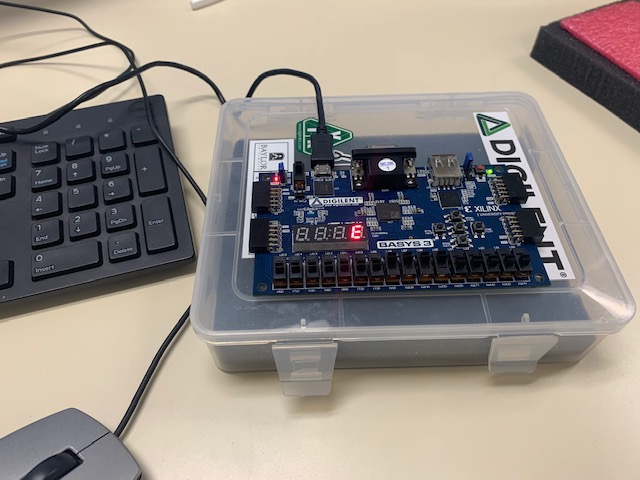
\includegraphics[width=.35\textwidth, trim=0cm 0cm 0cm 0cm,clip]{E}
	\caption{Here the board is showing a value on the first digit. (Value E)}
	\label{fig:Board-firstdigit}	
\end{figure}

\begin{figure}[ht]\centering
	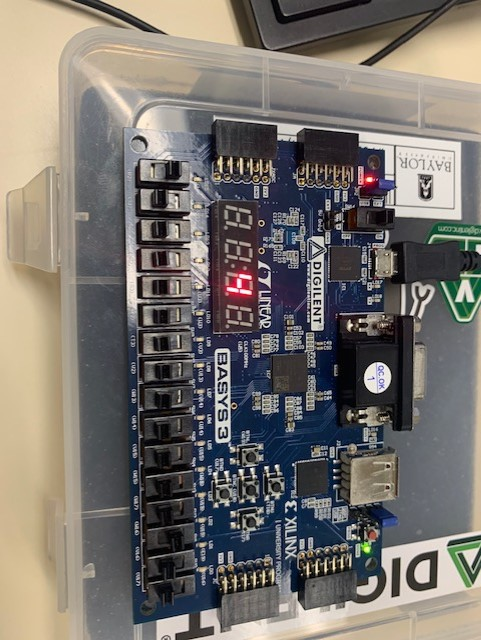
\includegraphics[width=0.25\textwidth, angle = 90, trim=0cm 0cm 0cm 0cm,clip]{4(2)}
	\caption{Here the board is showing a value on the second digit. (Value 4)}
	\label{fig:Board-seconddigit}	
\end{figure}

\subsection*{Errors}

	\begin{itemize}
		\item A very prominent error was that we could not seem to find the correct path for our 'out' variable in the sseg1.sv file.
		\item We then figured out that our statements in the sseg1test.sv were incorrect. Instead of repeating the same statements we did in the source code file, we decided it would be right to make an exclusive statement for all values of sw, and an.
		\item Both of these errors show that running simulations both constantly and consistently, strongly secure that your code is functioning properly throughout the process of writing it. If one were to write down all their code in one shot and process it at the very end there could be several errors (maybe even minor ones) that can really affect your outcome. It will be much easier to find the problem within your code if you run your simulations properly, also considering that you will be looking a smaller amount of code rather than the entirety of it.
		
		 
	\end{itemize}

\section*{Code}

\begin{lstlisting}[style=Verilog,
caption=mux2 4b Source Code,
label=mux2_4b:ex
]
`timescale 1ns / 1ps

module mux2_4b(
input [3:0] in0, in1, 
input sel, 
output [3:0] out
); 

assign out = sel? in0:in1; 

endmodule //mux2_4b
\end{lstlisting}

\begin{lstlisting}[style=Verilog,
caption=mux2 4b Test Code,
label=mux2 4b test:ex
]
`timescale 1ns / 1ps
// ELC 2137 - Lab6 - 02/20/2020
// Sebastian Lopez and Megan Gordon

module mux2_4b_test( );

reg [3:0] in0, in1;
reg sel; 
wire [3:0] out;

mux2_4b Test1(
.in0(in0), .in1(in1), .sel(sel),
.out(out)
); 

initial 
begin

sel = 1;
in0 = 0;
in1 = 1;
#10;  
sel = 1; 
in0 = 1; 
in1 = 0; 
#10; 
sel = 0;
in0 = 0;
in1 = 1;
#10;  
sel = 0; 
in0 = 1; 
in1 = 0; 
#10; 
$finish;

end  

endmodule//mux2_4b_test
\end{lstlisting}

\begin{lstlisting}[style=Verilog,
caption=Sseg Decoder Source Code,
label=sseg_decoder:ex
]
`timescale 1ns / 1ps
// ELC 2137 - Lab6 - 02/20/2020
// Sebastian Lopez and Megan Gordon

module sseg_decoder(
input [3:0] num,
output reg [6:0] sseg 
);

always @* 
case (num) 
4'h0: sseg = 7'b1000000;
4'h1: sseg = 7'b1111001;
4'h2: sseg = 7'b0100100;
4'h3: sseg = 7'b0110000;
4'h4: sseg = 7'b0011001;
4'h5: sseg = 7'b0010010;
4'h6: sseg = 7'b0000010;
4'h7: sseg = 7'b1111000;
4'h8: sseg = 7'b0000000;
4'h9: sseg = 7'b0010000;
4'hA: sseg = 7'b0001000;
4'hb: sseg = 7'b0000011;
4'hC: sseg = 7'b1000110;
4'hd: sseg = 7'b0100001;
4'hE: sseg = 7'b0000110;
4'hF: sseg = 7'b0001110;
endcase 
endmodule //sseg_decoder
\end{lstlisting}

\begin{lstlisting}[style=Verilog,
caption=Sseg Decoder Test Bench Code,
label=ssed_decoder_test:ex
]
`timescale 1ns / 1ps
// ELC 2137 - Lab6 - 02/20/2020
// Sebastian Lopez and Megan GordonS

module sseg_decoder_test();

reg [3:0] num; 
wire [6:0] sseg; 

integer i; 

sseg_decoder d1(
.num(num),
.sseg(sseg)
);  

initial begin 
for (i = 0; i <=8'hF; i=i+1) begin 
num = i; 
#10; 
end 
$finish; 
end 
endmodule //sseg_decoder_test
\end{lstlisting}

\begin{lstlisting}[style=Verilog,
caption=Sseg1 Source Code,
label=sseg1:ex
]
`timescale 1ns / 1ps
// ELC 2137 - Lab6 - 02/20/2020
// Sebastian Lopez and Megan Gordon

module sseg1(
input [15:0] sw, //switches 
output [3:0] an, // 7-segment digits
output [6:0] seg, // 7-seg segments
output dp // decimal point 
);

wire [3:0] out; 

not not1(an[1],sw[15]);
assign an[0] = sw[15];
assign an[3:2] = 3;
assign dp = 1; 

mux2_4b mux1(
.in0(sw[3:0]), .in1(sw[7:4]), .sel(sw[15]), 
.out(out) 
);

sseg_decoder sseg2(
.num(out),
.sseg(seg)
); 

endmodule //seg1
\end{lstlisting}

\begin{lstlisting}[style=Verilog,
caption=Sseg1 Test Bench Code,
label=sseg1_test:ex
]
`timescale 1ns / 1ps
// ELC 2137 - Lab6 - 02/20/2020
// Sebastian Lopez and Megan Gordon

module sseg1_test(
input [15:0] sw, //switches 
output [3:0] an, // 7-segment digits
output [6:0] seg, // 7-seg segments
output dp // decimal point 
);

wire [3:0] out; 

not not1(an[1],sw[15]);
assign an[0] = sw[15];
assign an[3:2] = 3;
assign dp = 1; 

mux2_4b mux1(
.in0(sw[3:0]), .in1(sw[7:4]), .sel(sw[15]), 
.out(out) 
);

sseg_decoder sseg2(
.num(out),
.sseg(seg)
); 

endmodule //seg1_test
\end{lstlisting}

\end{document}
